\chapter{(Linear) Group Actions}





\section{Group actions}


If $G$ is a group then we denote by $e \in G$ the neutral element and by $gh$ the composition of $g,h \in G$ and by $g^{-1}$ the inverse of $g \in G$.


\begin{defi}
 Given a group $G$ and a set $X$ then an \emph{action of $G$ on $X$} is a map
 \[
  \pi \colon G \times X \to X, (g,x) \to g.x,
 \]
 such that
 \begin{gather*}
  e.x = x \text{ and }
  (gh).x = g.(h.x)
 \end{gather*}
 for all $x \in X, g,h \in G$. We say then that \emph{$X$ is a $G$-set}.
\end{defi}


\begin{defi}
 Given a set $X$ let
 \[
  S(X) \coloneqq \{f \colon X \to X \mid f \text{ is bijective}\}.
 \]
 $S(X)$ is then a group with $fg \coloneqq f \circ g$ (composition of maps) for all $f,g \in S(X)$ and $e = \id_X$. $S(X)$ is called the \emph{symmetry group of $X$}.
\end{defi}


Given a group action $\pi \colon G \times X \to X$ any  $g \in G$ defines $\pi_g \in S(X)$ by setting
\[
 \pi_g(x) = \pi(g.x) \text{ for all } x \in X, g \in G.
\]


\begin{lem}\label{lem: G-actions = group homos G -> S(X)}
 Fix $G$ a group, $X$ a set. Then there is a 1:1-correspondence
 \[
 \begin{matrix}
    \left\{\text{$G$-actions on $X$}\right\}
  & \overset{1:1}{\longleftrightarrow}
  & \left\{\text{group homomorphisms $G \to S(X)$}\right\} \\
    \pi
  & \longmapsto
  & \hat{\pi} \\
    \mathring{\varphi}
  & \longmapsfrom
  & \varphi
  \end{matrix}
 \]
 where
 \[
  \hat{\pi}(g)(x) = g.x \text{ and } \mathring{\varphi}((g,x)) = \varphi(g)(x)
 \]
 for all $x \in X, g \in G$.
\end{lem}


From this Lemma we get the idea that group actions are ``the same'' as ``representing'' groups as permutation groups.


\begin{expls}
 Let $G$ be a group.
 \begin{enumerate}[label=\emph{\alph*)},leftmargin=*]
  \item
   $G$ acts on itself by left multiplication, i.e.
   \[
    g.x = gx \text{ for all } g \in G, x \in X=G.
   \]
   This is called the \emph{(left) regular action of $G$}.
  \item
   $G$ acts onto itself by right multiplication with the inverse, i.e
   \[
    g.x = xg^{-1} \text{ for all } g \in G, x \in X=G.
   \]
   This is called the \emph{right regular action}.
  \item
   $G$ acts onto itself by conjugation, i.e.
   \[
    g.x = gxg^{-1} \text{ for all }g \in G, x \in X=G.
   \]
  \item
   Let $X$ be any set. Then $g.x = x$ for all $g \in G, x \in X$ defines an action. This is called the \emph{trivial action} and $X$ is called a \emph{trivial $G$-set}.
  \item
   Let $X, Y$ be $G$-sets. Then
   \[
    \Maps(X,Y) = \{f \mid f \colon X \to Y\}
   \]
   is a $G$-set by setting
   \[
    (g.f)(x) = g.\left(f\left(g^{-1}.x\right)\right)
   \]
   for all $g \in G, x \in X$.
   In the special case that $Y$ is a trivial $G$-set this means $(g.f)(x) = f(g^{-1}.x)$ for all $g \in G, x \in X$.
  \item
   If $X, Y$ are $G$-sets then $X \times Y$ is a $G$-set via
   \[
    g.(x,y) = (g.x,g.y) \text{ for all } g \in G, x \in X, y \in Y.
   \]
  \item
   If $X$ is a set and $G = S(X)$, then $X$ is a $G$-set via $f.x = f(x)$ for all $f \in G, x \in X$.
 \end{enumerate}
\end{expls}


\begin{defi}
 Let $G$ be a group and $X, Y$ $G$-sets. Then $f \colon X \to Y$ is called \emph{$G$-equivariant} if
 \[
  f(g.x) = g.f(x)
 \]
 for all $g \in G, x \in X$. Denote
 \[
  \Hom_G(X,Y) = \{f \colon X \to Y \mid f \text{ is $G$-equivariant}\}.
 \]
\end{defi}


\begin{lem}
 Let $G$ be a group.
 \begin{enumerate}[label=\emph{\alph*)},leftmargin=*]
  \item
   If $X$ is a $G$-set, then $\id_X \in \Hom_G(X,X)$.
  \item
   If $X, Y, Z$ are $G$-sets with $f_1 \in \Hom_G(X,Y)$ and $f_2 \in \Hom_G(Y,Z)$ then $f_2 \circ f_1 \in \Hom_G(X,Z)$.
 \end{enumerate}
\end{lem}


\begin{expls}
 \begin{enumerate}[label=\emph{\alph*)},leftmargin=*]
  \item
   Let $G$ be a group and look at $G$ as a regular $G$-set. Then $f \colon G \to G$ is $G$-equivariant if and only if $f$ is given by right multiplication with some element $a \in G$ (i.e $f(g) = ga$ for all $g \in G$).
   \begin{proof}
    Assume there exists $a \in G$ such that $f(g) = ga$ for all $g \in G$. Then
    \[
     f(g.x) = f(gx) = (gx)a = g(xa) = g.f(x)
    \]
    for all $g, x \in G$. To show the other direction set $a \coloneqq f(e)$. Because $f$ is $G$-equivariant we then have
    \[
     f(g) = f(ge) = f(g.e) = g.f(e) = g.a = ga
    \]
    for all $g \in G$.
   \end{proof}
  \item
   If $X$ and $Y$ are trivial $G$-sets then $\Hom_G(X,Y) = \Maps(X,Y)$.
  \item
   If $X$ is a $G$-set and $Y$ is a trivial $G$-set then
   \[
    \Hom_G(X,Y) = \{f \colon X \to Y \mid f(g.x) = f(x) \text{ for all } g \in G, x \in X\}.
   \]
 \end{enumerate}
\end{expls}


The previous lemma shows that for a group $G$ the class of $G$-sets together with the $G$-equivariant maps between them form a category, which we will refer to as $\cGsets{G}$. So the objects in $\cGsets{G}$ are $G$-sets and
\[
 \Hom_{\cGsets{G}}(X,Y) = \Hom_G(X,Y)
\]
for any two $G$-sets $X$ and $Y$.


\begin{defi}
 Let $X$ be a $G$-set. We write
 \[
  X/G \coloneqq \{\text{orbits of $G$ in $X$}\}.
 \]
\end{defi}


\begin{note}
 There is an induced, but trivial action of $G$ on $X/G$ from the action of $G$ on $X$, and the canonical map
 \[
  \can \colon X \to X/G, x \mapsto \text{orbit of } x
 \]
 is $G$-equivariant, since
 \[
  \can(g.x) = \text{orbit of $g.x$} = \text{orbit of $x$} = \can(x) = g.\can(x)
 \]
 for all $g \in G, x \in X$.
\end{note}


\begin{defi}
 Let $X$ be a $G$-set. Then
 \[
  X^G \coloneqq \{\text{$G$-invariants of $X$}\} = \{x \in X \mid g.x = x \text{ for all } g \in G\}.
 \]
 The elements in $X^G$ are called \emph{$G$-invariants} or \emph{$G$ fix points}.
\end{defi}


\begin{lem}
 Let $X$ and $Y$ be $G$-sets and $f \colon X \to Y$ be $G$-equivariant. Then
 \[
  f(X^G) \subseteq Y^G.
 \]
\end{lem}
\begin{proof}
 For all $x \in X^G$ we have for all $g \in G$
 \[
  g.f(x) = f(g.x) = f(x).
 \]
 Thus $f(x) \subseteq Y^G$ for all $x \in X^G$.
\end{proof}


This lemma shows that a $G$-equivariant map $f \colon X \to Y$ between $G$-sets $X$ and $Y$ induces a map $f^G \colon X^G \to Y^G$ by restriction. It is clear that
\[
 \id_X^G = \id_{X^G}
\]
and that for any $G$-sets $X,Y,Z$ and $G$-equivariant maps $f \colon X \to Y$ and $g \colon Y \to Z$
\[
 (f \circ g)^G =  f^G \circ g^G.
\]
So we get a functor from $\cGsets{G}$ to $\cGsets{G}$ which sends every $G$-set $X$ to the corresponding trivial $G$-set $X^G$ and every $G$-equivariant map $f \colon X \to Y$ between $G$-sets $X$ and $Y$ to the $G$-equivariant $f^G \colon X^G \to Y^G$. (It is clear that $f^G$ is $G$-equivariant since both $X^G$ and $Y^G$ are trivial $G$-sets.)


\begin{lem}
 Let $X, Y$ be $G$-sets. Then $\Hom_G(X,Y) = \Maps(X,Y)^G$.
\end{lem}
\begin{proof}
 \begin{align*}
  f \in \Hom_G(X,Y)
  &\Leftrightarrow \forall g \in G, x \in X : f(g.x) = g.f(x) \\
  &\Leftrightarrow \forall g \in G, x \in X : f(g^{-1}.x) = g^{-1}.f(x) \\
  &\Leftrightarrow \forall g \in G, x \in X : g.f(g^{-1}.x) = f(x) \\
  &\Leftrightarrow \forall g \in G : g.f = f \\
  &\Leftrightarrow f \in \Maps(X,Y)^G.
  \qedhere
 \end{align*}
\end{proof}


\begin{defi}
 Let $X$ be a $G$-set, $k$ a field or a ring. A map $f \colon X \to k$ is called \emph{invariant} (or better \emph{$G$-invariant}) if
 \[
  f(x) = f(g^{-1}.x) \text{ for all } g \in G, x \in X.
 \]
\end{defi}


\begin{note}
 This agrees with the above definition of $f \in \Hom_G(X,k) = \Maps(X,k)^G$ if we consider $k$ as a trivial $G$-set.
\end{note}


\begin{lem}
 Let $X$ be a $G$-set, $k$ a field or a ring. Then $f \colon X \to k$ is invariant if and only if $f$ factors through $\can$, i.e.\ if the following diagram commutes.
 \tikzsetnextfilename{invariant_functions_factor_through_orbits}
 \begin{center}
 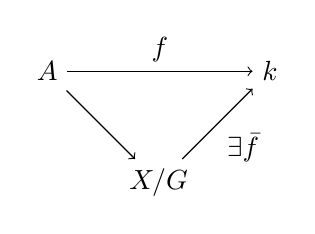
\begin{tikzpicture}[node distance = 2cm, auto]
  \node (A) {$A$};
  \node (XG) [below right of = A] {$X/G$};
  \node (k) [above right of = XG] {$k$};
  \draw[->] (A) to node {$f$} (k);
  \draw[->] (A) to node [swap] {$\can$} (XG);
  \draw[->] (XG) to node [swap] {$\exists\bar{f}$} (k);
 \end{tikzpicture}
 \end{center}
\end{lem}
\begin{proof}
 If $f$ is invariant then $f(x) = f(g^{-1}.x)$ for all $g \in G, x \in X$. Therefore $f$ is constant on orbits. Now define $\bar{f}(\mc{O}) = f(x)$ where $\mc{O}$ is an orbit and $x \in \mc{O}$.
 
 To show the other direction assume $f$ factors through $\can$. Then $f$ is constant on orbits, i.e.\ $f(x) = f(g.x)$ for all $g \in G, x \in X$, i.e.\ $f(x) = f(g^{-1}.x)$ for all $g \in G, x \in X$. Therefore $f$ is invariant.
\end{proof}


\begin{expl}
 Let $G = \Z/2 = \{e,s\}$ where $e$ is the neutral element and $s^2 = e$. Let $G$ act on $X = \R$ by $e.\lambda = \lambda$ and $s.\lambda = -\lambda$ for all $\lambda \in \R$. Set $k = \R$ and consider $\Maps(X,k) = \Maps(\R,\R)$. Any polynomial $p \in \R[X]$ can be viewed as an element in $\Maps(\R,\R)$. Take for example $p_n(X) = X^n$. We can ask ourselves which of the $p_n$’s is $G$-invariant. We need to check for which $n$ we have
 \[
  p_n(x) = p_n(s^{-1}.x) = p_n(s.x) = p_n(-x) \text{ for all } x \in \R.
 \]
 Since $p_n(X) = X^n$ we get that $p_n$ is $G$-invariant if and only if $n$ is even.
\end{expl}


\begin{lem}\label{lem: basis of Maps and Hom}
 Let $X$ be a finite $G$-set. Let $k$ be a field (or a ring).
 \begin{enumerate}[label=\emph{\alph*)},leftmargin=*]
  \item
   $\Maps(X,k)$ forms a $k$-vector space (resp. $k$-module) via pointwise addition and scalar multiplication.
  \item
   A $k$-basis of $\Maps(X,k)$ is given by $\{\chi_x \mid x \in X\}$ where
   \[
    \chi_x(y) =
    \begin{cases}
     1 & \text{if } x=y, \\
     0 & \text{otherwise}
    \end{cases}
   \]
   for all $y \in X$.
  \item
   $\Maps(X,k)^G = \Hom_G(X,k)$ is a $k$-vector subspace (resp. $k$-submodule) of $\Maps(X,k)$.
  \item
   A $k$-Basis of $\Maps(X,k)^G$ is given by $\{\chi_\mc{O} \mid \mc{O} \in X/G\}$ with
   \[
    \chi_\mc{O}(y) =
    \begin{cases}
     1 & \text{if } y \in \mc{O}, \\
     0 & \text{otherwise}
    \end{cases}
   \]
   for all $y \in X$.
 \end{enumerate}
\end{lem}
\begin{proof}
 \begin{enumerate}[label=\emph{\alph*)},leftmargin=*]
  \item
   This is left as an easy exercise for the reader.
  \item
   For $f \in \Maps(X,k)$ we have $f = \sum_{x \in X} f(x) \chi_x$. (Note that this sum is finite, hence defined.) This is true because for all $y \in X$ we have
   \[
    \sum_{x \in X} f(x) \chi_x(y) = f(y).
   \]
   This shows that the $\chi_x$'s generate $\Maps(X,k)$. They are linear independent since for $\alpha_x \in K, x \in X$ with $\sum_{x \in X} \alpha_x \chi_x = 0$ we have
   \[
    \alpha_y = \sum_{x \in X} \alpha_x \chi_x(y) = 0
   \]
   for all $y \in X$.
  \item
   We need to check that for all $f_1, f_2 \in \Maps(X,k)^G$ we have $f_1+f_2 \in \Maps(X,k)^G$ and that for all $f \in \Maps(X,k)^G$ and $\lambda \in k$ we have $\lambda f \in \Maps(X,k)^G$. This holds because
   \begin{align*}
    (g.(f_1+f_2))(x)
    &= (f_1+f_2)(g^{-1}.x) = f_1(g^{-1}.x) + f_2(g^{-1}.x) \\
    &= f_1(x) + f_2(x) = (f_1+f_2)(x) \text{ and} \\
    (g.(\lambda f))(x)
    &= (\lambda f)(g^{-1}.x) = \lambda (f(g^{-1}.x)) = \lambda f(x) = (\lambda f)(x)
   \end{align*}
   for all $x \in X, \lambda \in K$.
  \item
   Let $f \in \Maps(X,k)^G$ and $\mc{O}_1$, \dots, $\mc{O}_n$ be the orbits in $X$. Pick a representative $x_i \in \mc{O}_i$ for all $1 \leq i \leq n$. Then $f = \sum_{i=1}^n f(x_i) \chi_{\mc{O}_i}$. This adds because
   \[
    \sum_{i=1}^n f(x_i) \chi_{\mc{O}_i}(y) = f(x_j)
   \]
   for $j$ chosen such that $y \in \mc{O}_j$, i.e.\ $y = g^{-1}.x_j$ for some $g \in G$. We then have $f(y) = f(g^{-1}.x_j) = f(x_j)$. This shows that the $\chi_{\mc{O}_i}$’s generate $\Maps(X,k)^G$. The linear independence is clear (same argumentation as above).
  \qedhere
 \end{enumerate}
\end{proof}


If $X$ is an infinite $G$-set then we could replace $\Maps(X,k)$ by
\[
 kX \coloneqq \{f \in \Maps(X,k) \mid \supp(f) \text{ is finite}\}
\]
where
\[
 \supp(f) = \{x \in X \mid f(x) \neq 0\},
\]
is the \emph{support of $f$}, i.e
\[
 kX \coloneqq \{f \colon X \to k \mid f(x) \neq 0 \text{ for only finitely many } x \in X\}.
\]
Notice that for $f_1, f_2, f \in \Maps(X,k)$ we have
\[
 \supp(f_1+f_2) \subseteq \supp(f_1) \cup \supp(f_2)
\]
and
\[
 \supp(\lambda f) \subseteq \supp(f) \text{ for all } \lambda \in k.
\]
Therefore $kX$ with pointwise addition and scalar multiplication is again a $k$-vector space (resp. $k$-module).

Note that $\chi_x \in kX$ for all $x \in X$, since $\supp(\chi_x) = \{x\}$ is finite. Using the same argumentation as above we can show that $kX$ has a $k$-Basis $\{\chi_x \mid x \in X\}$, i.e.\ for alle $f \in kX$ we have $f = \sum_{x \in X} f(x) \chi_x$ (this sum is well-defined since only finitely many $f(x)$ are nonzero) and the $\chi_x$’s are linear independent.

Completely analogous to c) we have that
\begin{align*}
 kX^G
 &= (kX)^G = \left\{f \colon X \to k \,\middle|\, f \in kX, f \in \Maps(X,k)^G\right\} \\
 &= kX \cap \Maps(X,k)^G
\end{align*}Filter contributions
Additions
is a $k$-vector space (resp. $k$-submodule) inside $kX$. We claim that
\[
 \{\chi_\mc{O} \mid \mc{O} \in X/G, \mc{O} \text{ is finite}\}
\]
is a $k$-basis of $kX^G$.

To show this let $f \in kX^G$. Then $f = \sum_{i \in I} f(x_i) \chi_{\mc{O}_i}$ where $\{\mc{O}_i \mid i \in I\}$ is the set of orbits with finitely many elements and $x_i \in \mc{O}_i$ is a representative. Notice that if $f(x) \neq 0$ for some orbit $\mc{O}$ with infinitely many elements and $x \in \mc{O}$, then $\supp(f)$ is not finite, because $f$ is constant on orbits. Also notice that $f(x_i) \neq 0$ for only finitely many of the $x_i$’s because $\supp(f)$ is finite. Therefore the sum $f = \sum_{i \in I} f(x_i) \chi_{\mc{O}_i}$ is exactly the same as before. The linear independence of the $\chi_x$’s is clear.


\begin{lem}
 Let $X$ be a finite $G$-set. Assume that $X = X_1 \cup X_2$ with $X_1, X_2 \neq \emptyset$ and $X_1 \cap X_2 = \emptyset$ such that
 \begin{equation}\tag{\ensuremath{\ast}}\label{eqn:X_1 X_2 closed}
  g.x_1 \in X_1 \text{ and } g.x_2 \in X_2 \text{ for all } x_1 \in X_1, x_2 \in X_2, g \in G.
 \end{equation}
 Then
 \begin{enumerate}[label=\emph{\alph*)},leftmargin=*]
  \item
   $\Maps(X,k) \cong \Maps(X_1,k) \oplus \Maps(X_2, k)$ as $k$-vector spaces (resp. $k$-modules).
  \item
   $\Maps(X,k)^G \cong \Maps(X_1, k)^G \oplus \Maps(X_2, k)^G$ as $k$-vector spaces (resp. $k$-modules) where we have an induced action on both $\Maps(X_1, k)$ and $\Maps(X_2, k)$ from the $G$-action on $\Maps(X,k)$ via the isomorphism from a).
 \end{enumerate}
\end{lem}
\begin{proof}
 \begin{enumerate}[label=\emph{\alph*)},leftmargin=*]
  \item
   By Lemma \ref{lem: basis of Maps and Hom} we have a basis $B \coloneqq \{\chi_x \mid x \in X\}$ of $\Maps(X,k)$. Similarly $\Maps(X_i, k)$ has a basis $B_i \coloneqq \{\chi_x \mid x \in X_i\}$ for $i=1,2$. Since $B = B_1 \dotcup B_2$ we have $\Maps(X,k) \cong \Maps(X_1,k) \oplus \Maps(X_2,k)$ via
   \[
    \chi_x \mapsto
    \begin{cases}
     (\chi_x,0) & \text{ if } x \in X_1, \\
     (0,\chi_x) & \text{ if } x \in X_2.
    \end{cases}
   \]
  \item
   Let $f \in \Maps(X_1, k)$. Then define $(g.f)(x) = f(g^{-1}.x)$ for all $g \in G, x \in X_1$. Since $g^{-1}.x \in X_1$ for all $g \in G, x \in X_1$ this gives an induced action of $G$ on $\Maps(X,k)$ since \eqref{eqn:X_1 X_2 closed} holds. Similarly for $\Maps(X_2,k)$. In particular the isomorphism
   \[
    \Maps(X,k) \cong \Maps(X_1,k) \oplus \Maps(X_2,k)
   \]
   is $G$-equivariant. Thus we get the desired isomorphism by taking invariants on both sides.
  \qedhere
 \end{enumerate}
\end{proof}


\begin{expl}
 Assume $X$ is a finite trivial $G$-set. Since $X = \bigdotcup_{x \in X} \{x\}$ we have
 \[
  \Maps(X,k)
  \xlongequal{\text{Lemma \ref{lem: basis of Maps and Hom}}} \vspan \{\chi_x \mid x \in X\}
  = \bigoplus_{x \in X} k \chi_x
  = \bigoplus_{x \in X} \Maps(\{x\},k).
 \]
 In this case we have $\Maps(X,k)^G = \Maps(X,k)$ because the $G$-action on $k$ is trivial.
\end{expl}


\begin{expl}[\textbf{Warning!}]
 Given a $G$-set $X$ and a decomposition $\Maps(X,k) = V \oplus W$ into $k$-vector spaces (resp. $k$-modules) such that $g.v \in V, g.w \in W$ for all $g \in G, v \in V, w \in W$ this composition is not necessarily arising from a decomposition $X = X_1 \dotcup X_2$ as above.
 Let $G = \Z/2 = \{e,s\}$ with $s^2 = e$ and let $G$ act on itself by left multiplication, so $X = G$. Let $k$ be a field with $\kchar k \neq 2$.
 \begin{claim}
  There is no depcomposition $X = X_1 \cup X_2$ such that $X_1, X_2 \neq \emptyset$ and $X_1 \cap X_2 = \emptyset$ satisfying \eqref{eqn:X_1 X_2 closed}.
 \end{claim}
 \begin{proof}[Proof of claim]
  If such a decomposition would exist then $X_1 = \{e\}$ and $X_2 = \{s\}$ or $X_1 = \{s\}$ and $X_2 = \{e\}$. But since $s.e = se = s$ and $s.s = ss = e$ the condition \eqref{eqn:X_1 X_2 closed} fails, because we always have $s(X_1) \subseteq X_2$.
 \end{proof}
 Now consider $\Maps(X,k)$. By Lemma \ref{lem: basis of Maps and Hom} it has $\{\chi_e,\chi_s\}$ as a basis. Define
 \[
  b_1 \coloneqq \frac{\chi_e + \chi_s}{2} \text{ and } b_2 \coloneqq \frac{\chi_e - \chi_s}{2}.
 \]
 This is a basis of $\Maps(X,k)$. Since $s.\chi_e = \chi_s$ and $s.\chi_s = \chi_e$ we have
 \[
  s.b_1 = b_1 \text{ and } s.b_2 = -b_2.
 \]
 Therefore
 \[
  \Maps(X,k) = \vspan(b_1) \oplus \vspan(b_2)
 \]
 with $g.v \in V$ and $g.w \in W$ for all $g \in G, v \in V, w \in W$.
\end{expl}


\begin{lem}\label{lem: group action by ring automorphisms}
 Assume $G$ acts on $R$ where $R$ is a set but also a ring. Assume $G$ acts by ring automorphisms (i.e.\ if $\pi \colon G \times R \to R$ is the action then $\pi_g \colon r \mapsto g.r$ is an ring automorphism of $R$ for all $g \in G$). Then $R^G = \{\text{$G$-invariants of $R$}\}$ forms again a ring, namely a subring of $R$.
\end{lem}
\begin{proof}
 We need to show that for all $r_1, r_2 \in R^G$ we have $r_1 + r_2 \in R^G$ and $r_1 r_2 \in R^G$. This is true because
 \[
  g.(r_1 + r_2) = \pi_g(r_1 + r_2) = \pi_g(r_1) + \pi_g(r_2) = g.r_1 + g.r_2 = r_1 + r_2
 \]
 and
 \[
  g.(r_1 r_2) = \pi_g(r_1 r_2) = \pi_g(r_1) \pi_g(r_2) = (g.r_1)(g.r_2) = r_1 r_2
 \]
 for all $g \in G$.
\end{proof}


\begin{rem}
 Here rings don't necessarily have an 1-element.
\end{rem}


\begin{expl}
 Let $X$ be a $G$-set and $k$ a field (or a ring). Then:
 \begin{enumerate}[label=\emph{\alph*)},leftmargin=*]
  \item
   $\Maps(X,k)$ forms a ring via pointwise addition and multiplication.
  \item
   The usual $G$-action on $\Maps(X,k)$ (i.e.\ $(g.f)(x) = f(g^{-1}.x)$ for each $g \in G, x \in X$) is an action by ring automorphisms. Hence $\Maps(X,k)^G$ is a subring of $\Maps(X,k)$.
 \end{enumerate}
 \begin{proof}
  \begin{enumerate}[label=\emph{\alph*)},leftmargin=*]
   \item
    We leave this as an exercise to the reader.
   \item
    For all $f_1, f_2 \in \Maps(X,k), x \in X$ we have
    \begin{align*}
     (g.(f_1+f_2))(x) &= \left(f_1+f_2)(g^{-1}.x\right) = f_1\left(g^{-1}.x\right) + f_2\left(g^{-1}.x\right) \\
     &= (g.f_1)(x) + (g.f_2)(x) = ((g.f_1)+(g.f_2))(x)
    \end{align*}
    and
    \begin{align*}
     (g.(f_1 f_2))(x) &= (f_1 f_2)\left(g^{-1}.x\right) = f_1\left(g^{-1}.x\right) f_2\left(g^{-1}.x\right) \\
     &= (g.f_1)(x) (g.f_2)(x) = ((g.f_1)(g.f_2))(x),
    \end{align*}
    so $G$ acts by ring homomorphisms. Since $\pi_g$ has the inverse $\pi_{g^{-1}}$ these homomorphisms are automatically automorphisms. The rest is a consequence of Lemma \ref{lem: group action by ring automorphisms}.
   \qedhere
  \end{enumerate}
 \end{proof}
\end{expl}


\begin{rem}
 Similar statements hold for $kX$ and $(kX)^G$ (with the same proofs).
\end{rem}


\begin{defi}
 Let $G$ and $H$ be groups, $X$ a set such that $\pi \colon G \times X \to X$ and $\pi' \colon H \times X \to X$ are group actions (i.e.\ $X$ is a $G$-set and $H$-set). Then the actions commute if
 \[
  h.(g.x) = g.(h.x)
 \]
 for all $g \in G, h \in H, x \in X$.
\end{defi}


\begin{rem}
 In this case we have that $\pi_g$ is an $H$-equivariant map for all $g \in G$ and $\pi'_h$ is an $G$-equivariant map for all $h \in H$, because
 \[
  g.\pi_h(x) = \pi_g(h.x) = g.(h.x) = h.(g.x) = h.\pi_g(x) = \pi_h(g.x)
 \]
 for all $g \in G, h \in H$.
\end{rem}


\begin{expls}
 \begin{enumerate}[label=\emph{\alph*)},leftmargin=*]
  \item
   Let $G$ be a group. Then the left regular action and the right regular action of $G$ on $G$ commute.
  \item
   Let $G$ be a group. The left regular action and conjugation action of $G$ on $G$ commute if and only if $G$ is abelian: If $.$ denotes the left regular action and $*$ the conjugation then
   \begin{align*}
    g_1*(g_2.x) &= g_1 (g_2 x) g_1^{-1} = g_1 g_2 x g_1^{-1} \text{ and} \tag{\ensuremath{\ast}}\\
    g_2.(g_1*x) &= g_2 \left(g_1 x g_1^{-1}\right) = g_2 g_1 x g_1^{-1} \tag{\ensuremath{\ast\ast}},
   \end{align*}
   for all $g_1, g_2, x \in G$. So
   \begin{align*}
    (\ast) = (\ast\ast) \text{ for all } g_1, g_2, x \in G
    &\Leftrightarrow g_1 g_2 = g_2 g_1 \text{ for all } g_1, g_2 \in G \\
    &\Leftrightarrow \text{$G$ is abelian}.
   \end{align*}
  \item
   Let $G = \GL(2,\R)$. $G$ acts on $\R^2$ in the natural way. Consider
   \[
    H \coloneqq \left\{ \vect{\lambda&0\\0&\lambda} \,\middle|\, \lambda \in \R, \lambda \neq 0 \right\} \subseteq \GL(2,\R).
   \]
   Then $H$ acts on $\R^2$ by restriction of the $G$-action. The two actions commute since $gh = hg$ for all $g \in G, h \in H$. (Notice that $H$ is the center of $G$.)
 \end{enumerate}
\end{expls}





\section{Representations of groups.}


\begin{defi}
 Let $G$ be a group, $V$ a $k$-vector space and $\pi \colon G \times V \to V$ be a group action. The action is linear if $\pi_g \colon V \to V, v \mapsto g.v$ is $k$-linear for all $g \in G$. $V$ is then called a $G$-space.
\end{defi}


\begin{expl}
 The natural action of $\GL(2,\R)$ on $\R^2$ in the previous example is $\R$-linear.
\end{expl}


For a $k$-vector space $V$ we set
\[
 \GL(V) \coloneqq \{f \colon V \to V \mid f \text{ is $k$-linear and invertible}\}.
\]


\begin{lem}
 Let $G$ be a group and $V$ a $k$-vector space. Then there is a 1:1-correspondence
 \[
    \left\{\text{linear $G$-actions on $X$}\right\}
  \overset{1:1}{\longleftrightarrow}
  \left\{\text{group homomorphisms $G \to \GL(V)$}\right\}.
 \]
\end{lem}
\begin{proof}
 As in Lemma \ref{lem: G-actions = group homos G -> S(X)}.
\end{proof}


\begin{rem}
 A $G$-space $V$ or equivalently a vector space $V$ with a group homomorphism $G \to \GL(V)$ is called a representation of $G$.
\end{rem}


\begin{expls}
 \begin{enumerate}[label=\emph{\alph*)},leftmargin=*]
  \item
   Let $V$ be a $k$-vector space. Then $\GL(V)$ acts linearly on $V$ in a natural way. (The action corresponds to the group homomorphism $\id_{\GL(V)} \colon \GL(V) \to \GL(V)$.)
  \item
   If $X$ is a $G$-set then $kX$ is naturally a $G$-space by setting
   \[
    g.\left(\sum_{x \in X} a_x \chi_x\right) = \sum_{x \in X} a_x \chi_{g.x}
   \]
   where almost all $a_x$ are zero. This agrees with the previous action on $kX$, because
   \[
    (g.\chi_x)(y)
    = \chi_x(g^{-1}.y)
    = \begin{cases} 1 & \text{if } x = g^{-1}.y, \\ 0 & \text{otherwise}, \end{cases}
    = \begin{cases} 1 & \text{if } g.x = y, \\ 0 & \text{otherwise}, \end{cases}
    = \chi_{g.x}(y)
   \]
   for all $y \in X$.
  \item
   Let $V$ and $W$ be $G$-spaces over the same field. Then the $G$-action on $\Maps(V,W)$ induces a linear action of $G$ on $\Hom(V,W)$. Since $G$ acts linearly on $V$ and $W$ we know that for every $g \in G$ the maps $\pi_g \colon V \to V, v \mapsto g.v$ and $\tau_g \colon W \to W, w \mapsto g.w$ are linearly. With this we find that for every $g \in G$ and $f \in \Hom(V,W)$ we have
   \[
    g.f = \tau_g \circ f \circ \pi_{g^{-1}} \in \Hom(V,W).
   \]
   Therefore $\Hom(V,W)$ is closed under the action of $G$ on $\Maps(V,W)$. Since the composition above is $k$-linear in $f$ it also follows that the action is linear on $\Hom(V,W)$.
  \item
   Let $V$ and $W$ be $G$-spaces over the same field. Then $V \oplus W$ and $V \otimes W$ are $G$-spaces via
   \begin{align*}
    g.(v,w) &= (g.v,g.w) \text{ and }  \tag{1} \\
    g.(v \otimes w) &= (g.v) \otimes (g.w) \tag{2}
   \end{align*}
   for all $v \in V, w \in W, g \in G$. 
   Notice that the linear action on $V \otimes W$ is induces by the linear action on $V \times W$: If $\pi \colon G \times V \to V$ is the action on $V$ and $\pi' \colon G \times W \to W$ is the action on $W$ then the action $\tau \colon G \times (V \times W) \to V \times W$ defined by (1) is given by $\tau_g = \pi_g \times \pi'_g$ for all $g \in G$. The action $\tau' \colon G \times (V \otimes W) \to V \otimes W$ defined by (2) is then given by $\tau_g = \pi_g \otimes \pi'_g$ for all $g \in G$. So $\tau'$ it is the unique action making the diagram in figure \ref{fig: action on product and tensor} commute for all $g \in G$.
   \tikzsetnextfilename{tensor_product_of_representations}
   \begin{figure}\label{fig: action on product and tensor}\centering
    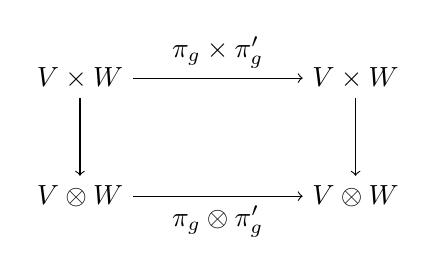
\begin{tikzpicture}[node distance = 3.5cm, auto]
     % the nodes
     \node (V times W) {$V \times W$};
     \node (V times W 2) [right of = V times W] {$V \times W$};
     \node (V tensor W) [below of = V times W, node distance = 1.5cm] {$V \otimes W$};
     \node (V tensor W 2) [right of = V tensor W] {$V \otimes W$};
     % the arrows
     \draw[->] (V times W) to node {$\pi_g \times \pi'_g$} (V times W 2);
     \draw[->] (V times W) to (V tensor W);
     \draw[->] (V times W 2) to (V tensor W 2);
     \draw[->] (V tensor W) to node [swap] {$\pi_g \otimes \pi'_g$} (V tensor W 2);
    \end{tikzpicture}
    \caption{The action of $g \in G$ on $V \times W$ and $V \otimes W$.}
   \end{figure}
   If $v_1$, \dots, $v_n$ is a basis of $V$ and $w_1$, \dots, $w_m$ a basis of $W$ we can write the action of $g \in G$ on $V$, resp. $W$, as a matrix $A$, resp. $B$. The actions $(1)$ and $(2)$ are then given by matrices
   \[
    \begin{pmatrix}
     A & 0 \\
     0 & B
    \end{pmatrix}
    \text{ and }
    \begin{pmatrix}
     a_{11} B & a_{12} B & \cdots & a_{1m} B \\
     a_{21} B & a_{22} B & \cdots & a_{2m} B \\
      \vdots  &  \vdots  & \ddots &  \vdots  \\
     a_{n1} B & a_{n2} B & \cdots & a_{nm} B
    \end{pmatrix}
   \]
   with respect to the basis $v_1$, \dots, $v_n$, $w_1$, \dots, $w_m$ of $V \oplus W$ and the basis $v_1 \otimes w_1$, $v_1 \otimes w_2$, \dots, $v_n \otimes w_m$ of $V \otimes W$.
  \item
   Let $V$ and $W$ be $G$-spaces over the same field. Then $V \vee W$ and $V \wedge W$ can also be given the structure of a $G$-space in the same way as $V \otimes W$.
 \end{enumerate}
\end{expls}


\begin{defi}
  Let $V$ ba a $G$-space or equivalently a representation of $G$.

  A \emph{subrepresentation} of $V$ is a vector subspace $U$ of $V$ such that $g.u \in U$ for all $u \in U, g \in G$. A subrepresentation $U$ of $V$ is \emph{proper} if $U \neq V$.
  
  $V$ is \emph{indecomposable} if it can’t be written as $V = U_1 \oplus U_2$ where $U_1, U_2$ are proper subrepresentations of $V$.
  
  $V$ is \emph{irreducible} if it is nonzero has no nontrivial proper subrepresentation.
\end{defi}

It is clear that every irreducible representation is also indecomposable. The converse is not true in general as the following example shows.

\begin{expl}
 Let
 \[
  G \coloneqq \left\{ \vect{a&b\\0&c} \,\middle|\, a,b,c \in \C \text{ and } a, c \neq 0 \right\}.
 \]
 $G$ acts on $V \coloneqq \C^2$ in the natural way. Notice that $V$ is not irreducible because $U \coloneqq \vspan(e_1)$ is a subrepresentation since
 \[
  \vect{a&b\\0&c} \vect{\alpha\\0} = \vect{\alpha a\\0} \in U
 \]
 for all $\alpha \in \C$. But $V$ is indecomposible because $U$ is the unique $1$-dimensional subrepresentation of $V$.  Therefore there exist no proper subrepresentations $U_1, U_2$ of $V$ with $V = U_1 \oplus U_2$. To show that $U$ is the unique $1$-dimensional subrepresentation of $V$ let $W$ be an $1$-dimensional subrepresentation of $V$. Then
 \[
  W = \vspan\left\{ \vect{\alpha\\\beta} \right\} \text{ for some } \vect{\alpha\\\beta} \in \C^2.
 \]
 Because $W$ is a subrepresentation of $V$ we have
 \[
  \vect{1&1\\0&1} \vect{\alpha\\\beta} = \vect{\alpha+\beta\\\beta} \in W.
 \]
 and therefore
 \[
  \vect{\beta\\0} \in W.
 \]
 So we find that
 \[
  \vect{1\\0} \in W
 \]
 and thus
 \[
  W = \vspan\left\{\vect{1\\0}\right\} = U.
 \]
\end{expl}


\begin{warn}
 As seen above subrepresentations have not always complements which are again subrepresentations.
\end{warn}


\begin{lem}\label{lem: direct sum and invariants commute}
 Let $G$ be a group.
 \begin{enumerate}[label=\emph{\alph*)},leftmargin=*]
  \item
   Given a representation $V$ of $G$ the subset $V^G \subseteq V$ is a (trivial) subrepresentation of $V$.
  \item
   Given a collection $V_i$, $i \in I$ of representations of $G$ we have
   \[
    \left( \bigoplus_{i \in I} V_i \right)^G = \bigoplus_{i \in I} V_i^G.
   \]
 \end{enumerate}
\end{lem}
\begin{proof}
 \begin{enumerate}[label=\emph{\alph*)},leftmargin=*]
  \item
   Since $G$ acts trivially on $V^G$ we only need to check that that $V^G$ is a vector subspace of $V$. This holds becaues $\pi_g \colon V \to V, v \mapsto g.v$ is linear for every $g \in G$ and
   \[
    V^G = \bigcap_{g \in G} \ker(\pi_g - \id_V).
   \]
  \item
   Let $v \in \left( \bigoplus_{i \in I} V_i \right)^G$ with $v = \sum_{i \in I} v_i$ where $v_i \in V_i$ for every $i \in I$ and $v_i = 0$ for all but finitely many $i \in I$. Because $V_i$ is a subrepresentation of $\bigoplus_{i \in I} V_i$ for every $i \in I$ and $G$ acts linearly on $\bigoplus_{i \in I} V_i$ we find that for every $g \in G$
   \[
    \sum_{i \in I} v_i
    = v
    = g.v
    = g.\left( \sum_{i \in I} v_i \right)
    = \sum_{i \in I} g.v_i.
   \]
   Because the sum $\bigoplus_{i \in I} V_i$ is direct we find that $g.v_i = v_i$ for every $g \in G$, $i \in I$. So $v_i \in V_i^G$ for every $i \in I$. Thus $v \in \bigoplus_{i \in I} V_i^G$ and therefore
   \[
    \left( \bigoplus_{i \in I} V_i \right)^G \subseteq \bigoplus_{i \in I} V_i^G.
   \]
   The other inclusion is obvious.
 \end{enumerate}
\end{proof}





\section{Group algebras}


\begin{defi}
 Let $k$ be a field (or a ring) and $G$ a group. Then the \emph{group algebra of $G$ over $k$} is the $k$-algebra with $1$ given by the $k$-vector space
 \[
  kG \coloneqq \{f \colon G \to k \mid f(g) \neq 0 \text{ for only finitely many } g \in G\}
 \]
 with (1) pointwise addition and scalar multiplication and (2) multiplication given by convolution, i.e.\
 \[
  (f_1 \cdot f_2)(x) = \sum_{y \in G} f_1(y) f_2\left(y^{-1}x\right)
 \]
 for all $f_1, f_2 \in kG, x \in G$.
\end{defi}

The unit of the group algebra is given by the function $\chi_e$. We leave it as an exercise to the reader to check that this is a $k$-algebra.

To make it easier to work with this algebra we provide another way to think about it:

We can write $f \in kG$ as $f = \sum_{g \in G} a_g \chi_g$ with $a_g \in k$ for all $g \in G$ where almost all $a_g$ are zero. We also write $\sum_{g \in G} a_g g$ as a shorter notation for the sum above. The addition and scalar multiplication as in (1) can then be written as
\begin{gather*}
 \left( \sum_{g \in G} a_g g \right) + \left( \sum_{g \in G} b_g g \right) = \sum_{g \in G} (a_g+b_g) g \text{ and}\\
 \lambda \left( \sum_{g \in G} a_g g \right) = \sum_{g \in G} (\lambda a_g) g \text{ for all } \lambda \in k
\end{gather*}
and the multiplication (2) as
\[
 \left( \sum_{g \in G} a_g g \right) \cdot \left( \sum_{g \in G} b_g g \right)
 = \sum_{h, g \in G} a_g b_{g^{-1}h} h
 = \sum_{g, g' \in G} a_g b_{g'} (g g').
\]
To verify that this multiplication is equivalent to (2) it is enough to check this on a basis, because both multiplications are $k$-bilinear.

Multiplying in the first way gives us
\begin{align*}
 \left( \chi_{g_1} \cdot \chi_{g_2} \right)(h)
 &= \sum_{y \in G} \chi_{g_1}(y) \chi_{g_2}\left(y^{-1} h\right)
 = \chi_{g_2}\left(g_1^{-1}h\right) \\
 &= \begin{cases} 1 & \text{if } g_2 = g_1^{-1}h, \\ 0 & \text{otherwise}, \end{cases}
 = \begin{cases} 1 & \text{if } g_1 g_2 = h, \\ 0 & \text{otherwise}, \end{cases}
 = \chi_{g_1 g_2}(h),
\end{align*}
so $\chi_{g_1} \cdot \chi_{g_2} = \chi_{g_1 g_2}$ for all $g_1, g_2 \in G$.
For multiplication in the second way we write $\chi_g$ as $\sum_{h \in G} a^g_h h$ where
\[
 a^g_h = \begin{cases} 1 & \text{if } h = g, \\ 0 & \text{otherwise}, \end{cases}
\]
for all $g \in G$. For $g_1, g_2 \in G$ multiplying $\chi_{g_1}$ and $\chi_{g_2}$ in the second way gives us
\[
 \chi_{g_1} \cdot \chi_{g_2}
 = \left( \sum_{g \in G} a^{g_1}_g g \right) \cdot \left( \sum_{g \in G} a^{g_2}_g g \right)
 = \sum_{g,g' \in G} a^{g_1}_g a^{g_2}_{g'} (g g')
 = (g_1 g_2)
 = \chi_{g_1 g_2}.
\]
This shows that the multiplications the same.

So we can think of the multiplication in $kG$ as the $k$-bilinear extension of the multiplication in $G$. Also note that $kG$ is commutative if and only if $G$ is commutative.


\begin{lem}
 Let $G$ be a group and $V$ a $k$-vector space. Then there is a 1:1-correspondence
 \[
 \begin{matrix}
    \left\{\text{linear $G$-actions on $V$}\right\}
  & \overset{1:1}{\longleftrightarrow}
  & \left\{\text{$kG$-module structures on $V$}\right\} \\
    \pi
  & \longmapsto
  & \hat{\pi}
  \end{matrix}
 \]
 where $\pi \colon G \times V \to V, (g,v) \mapsto g.v$ is a linear group action and
 \[
  \hat{\pi} \colon kG \times V \to V, \left(\sum_{g \in G} a_g g, v\right) \mapsto \sum_{g \in G} a_g (g.v).
 \]
\end{lem}
\begin{proof}
 The proof is left as an exercise to the reader and will most likely appear on some exercise sheet in the future.
\end{proof}





\section{Morphism of representations}


\begin{defi}
Let $G$ be a group, $k$ any field and $V,W$ representations of $G$. A map $f \colon V \to W$ is called a \emph{morphism of $G$-spaces} or \emph{morphism of representations of $G$} if $f$ is $k$-linear and $G$-equivariant. An \emph{isomorphism of representations} is an morphism of representations which is also invertible as a $k$-linear map. We call $V$ and $W$ \emph{isomorphic (as representations of $G$)}, denoted by $V \cong W$, if there exists an isomorphism of representations between $V$ and $W$. We denote
\[
 \Hom_G(V,W) = \{f \colon V \to W \mid f \text{ is a morphism of representations}\}.
\]
\end{defi}


\begin{rem}
 If $f \colon V \to W$ is an isomorphism of representations, then its linear inverse $f^{-1}$ is again a morphism of representations, because $f^{-1}$ is linear by definition and it is $G$-equivariant, because for all $g \in G, v \in V$
 \[
  f\left(f^{-1}(g.v)\right) = g.v = g.f\left(f^{-1}(v)\right) = f\left(g.f^{-1}(v)\right)
 \]
 and $f$ is bijective (and therefore injective).
\end{rem}


\begin{rem}
 If $V$ and $W$ are representations of $G$ then $\Hom_G(V,W)$ is a $k$-vector space via pointwise addition und scalar multiplication. (This will be on one of the exercise sheets.)
\end{rem}


\begin{lem}\label{lem: composition of morphisms of representations}
 Let $G$ be a group.
 \begin{enumerate}[label=\emph{\alph*)},leftmargin=*]
  \item
   $\id_V \colon V \to V$ is a morphism of representations for any representation $V$ of $G$.
  \item
   If $f \colon V \to W$  and $g \colon W \to Z$ are morphism of representations of $G$, then $g \circ f \colon V \to Z$ is a morphism of representations.
 \end{enumerate}
\end{lem}
\begin{proof}
 Part a) is trivial. It is also clear that $g \circ f$ is $k$-linear and $G$-equivariant (see the proof in chapter I for $G$-sets).
\end{proof}


The previous lemma shows that for any group $G$ and field $k$ the class of representations of $G$ over $k$ together with morphisms of representations between them form a category, which we will denote by $\cRep{k}{G}$. As before we have a functor from $\cRep{k}{G}$ to $\cRep{k}{G}$ which sends $V$ to $V^G$ and every morphism of representations $f \colon V \to W$ to the restriction $f^G \colon V^G \to W^G$.


\begin{lem}\label{lem: ker and im subrepresentations}
 Let $V,W$ be representations of a group $G$, $f \in \Hom_G(V,W)$. Then $\ker f$ is a subrepresentation of $V$ and $\im f$ is a subrepresentation of $W$.
\end{lem}
\begin{proof}
 Since $f$ is linear, $\ker f$ is a vector subspace of $V$ and $\im f$ is a vector subspace of $W$.
 
 Let $x \in \ker f$. Then $f(g.x) = g.f(x) = g.0 = 0$ for all $g \in G$, because $G$ acts linear. So $g.x \in \ker f$ for all $g \in G, x \in \ker f$.
 
 Let $y = f(x) \in \im f$. Then $g.y = g.f(x) = f(g.x) \in \im f$ for all $g \in G$.
\end{proof}


\begin{lem}[Schur’s Lemma]
 Let $k$ be a field, $G$ a group, $V$ and $W$ irreducible representations of $G$.
 \begin{enumerate}[label=\emph{\alph*)},leftmargin=*]
  \item
   We have $\Hom_G(V,W) = 0$ if $V \not\cong W$ and $\Hom_G(V,W) \not\cong 0$ if $V \cong W$, and every non zero morphism is an isomorphism.
  \item
   $\Hom_G(V,V)$ is a divison ring / skew field (i.e.\ we have $1 \neq 0$ and every non zero endomorphism is invertible).
  \item
   In the special case that $k$ is algebraically closed (e.g. $k = \C$) and $V$ and $W$ are both finite dimensional we have that
   \[
    \Hom_G(V,W) \cong
    \begin{cases}
     k & \text{if } V \cong W, \\
     0 & \text{if } V \not\cong W,
    \end{cases}
   \]
   as vector spaces.
 \end{enumerate}
\end{lem}
\begin{proof}
 \begin{enumerate}[label=\emph{\alph*)},leftmargin=*]
  \item 
   Assume $0 \neq f \in \Hom_G(V,W)$. Then by Lemma \ref{lem: ker and im subrepresentations} $\ker f$ and $\im f$ are subrepresentations of $V$, resp. $W$. Since $V$ and $W$ are irreducible we have that
   \[
    \ker f = 0 \text{ or } \ker f = V \quad \text{and} \quad \im f = 0 \text{ or } \im f = W.
   \]
   Since $f \neq 0$ we have $\ker f \neq V$ and $\im f \neq 0$. So $\ker f = 0$ and $\im f = W$.
  \item
   It is clear that $V \cong V$, so it follows from a).
  \item
   Assume $\alpha, \beta \in \Hom_G(V,W)$ where $V \cong W$ and $\alpha \neq 0$. It is enough to show that there exists some $\lambda \in k$ such that $\beta = \lambda \alpha$. Consider the morphism $\alpha^{-1} \beta \in \Hom_G(V,W)$ (this is well defined since we know from a) that $\alpha$ is invertible and $\alpha^{-1}$ is again a morphism of representations by the previous Remark, hence $\alpha^{-1} \beta \in \Hom_G(V,W)$ by lemma \ref{lem: composition of morphisms of representations}).
   
   Because $k$ is algebraically closed $\alpha^{-1} \beta$ has some eigenvalue $\lambda \in k$. By \mbox{lemma \ref{lem: ker and im subrepresentations}}
   \[
    K \coloneqq \ker(\alpha^{-1} \beta - \lambda \id_V)
   \]
   is a subrepresentation of $V$. Since $V$ is irreducible and $K \neq 0$ (because $\lambda$ is an eigenvalue of $\alpha^{-1} \beta$) we have $K = V$. So $\alpha^{-1} \beta = \lambda \id_V$ and therefore $\beta = \lambda \alpha$.
  \qedhere
 \end{enumerate}
\end{proof}


\begin{cor}
 Let $k$ be an algebraically closed field, $G$ an abelian group and $V$ a finite-dimensional irreducible representation of $G$ over $k$. Then $\dim_k V = 1$.
\end{cor}
\begin{proof}
 For every $g \in G$ the map
 \[
  \pi_g \colon V \to V, v \mapsto g.v
 \]
 is $G$-equivariant, since for all $h \in G$
 \[
  \pi_g \circ \pi_h = \pi_{gh} = \pi_{hg} = \pi_h \circ \pi_g.
 \]
 So $\pi_g \in \End_G(V)$ for all $g \in G$. By Schur’s Lemma we find that $\End_G(V) \cong k$, and so every $g \in G$ acts by multiplication with some scalar $\lambda \in k$. So every one-dimensional vector subspace of $V$ is an irreducible subrepresentation of $V$. Since $V$ is already irreducible itself we find that $V$ is one-dimensional.
\end{proof}


\begin{rem}
 Assume $k$ is an algebraically closed field and $V$ a finite dimensional irreducible representation of some group $G$. Then
 \[
  \End_G(V \oplus \dotsb \oplus V)
  \coloneqq \Hom_G(V \oplus \dotsb \oplus V, V \oplus \dotsb \oplus V)
  \cong \Mat(n \times n, k)
 \]
 is an isomorphism of rings by Schur’s lemma part c).
 
 More general: Let $V_1$, \dots, $V_r$ be pairwise non-isomorphic irreducible finite dimensioal representations of some group $G$ and $W_i \coloneqq V_i^{n_i}$. Then
 \begin{align*}
  \End_G(W_1 \oplus \dotsb \oplus W_r)
  &= \End(V_1^{n_1} \oplus \dotsb \oplus V_n^{n_r}) \\
  &\cong \End(V_1^{n_1}) \oplus \dotsb \oplus \End(V_r^{n_r}) \\
  &\cong \Mat(n_1 \times n_1, k) \oplus \dotsb \oplus \Mat(n_r \times n_r, k)
 \end{align*}
 as rings.
\end{rem}


\begin{defi}
 Let $G$ be a group. A representation $V$ of $G$ (over a field $k$) is \emph{completely reducible} if
 \[
  V \cong V_1 \oplus \dotsb \oplus V_r
 \]
 for some irreducible representations $V_1$, \dots, $V_r$.
\end{defi}


\begin{rem}
 Not every representation is completely reducible, even if $k$ is algebraically closed. Consider, for example,
 \[
  G \coloneqq \left\{\vect{a & b \\ 0 & c} \,\middle|\, a,b,c \in \C \text{ and } a,c \neq 0\right\}
  \subseteq \GL_2(\C)
 \]
 and the natural representation of $G$ on $\C^2$. We saw earlier that $U \coloneqq \vspan(e_1)$ gives a subrepresentation and it’s the only $1$-dimensional subrepresentation. So the representation is not irreducible, but at the same time not isomorphic to a direct sum of irreducible representations.
\end{rem}


\begin{thrm}[Maschke’s theorem]
 Let $G$ be a finite group and $k$ a field such that $\kchar k \nmid |G|$ (in particular $\kchar k = 0$ is allowed). Then any finite dimensional representation of $G$ over $k$ is completely reducible.
\end{thrm}
\begin{proof}
 It is enough to show that every subrepresentation $U$ of $V$ has a complement $W$ which is again a subrepresentation, i.e.\ $V = U \oplus W$ as representations.
 
 Given our subrepresentation $U$ choose a complement $W$ as a vector space. Then $V = U \oplus W$ as vector spaces. Let $p \colon V \to U$ be the orthogonal projection onto $U$. ($p$ is not necessarily $G$-equivariant but only a linear map.) We know that $\im p = U$. We define $\hat{p} \colon V \to U$ as
 \[
  \hat{p}(v) \coloneqq \frac{1}{|G|} \sum_{g \in G} g^{-1}.p(g.v).
 \]

This is well defined since $|G| < \infty$ and $1/|G|$ is defined, because $\kchar k \nmid |G|$. Note that $\im \hat{p} \subseteq U$, since $p(g.v) \in U$ and $U$ is a subrepresentation, hence $g^{-1}.p(g.v) \in U$ for all $g \in G, v \in V$.

It is clear that $\hat{p}(u) = u$ for all $u \in U$ because
\[
 \hat{p}(u)
 = \frac{1}{|G|} \sum_{g \in G} g^{-1}.p(g.u)
 = \frac{1}{|G|} \sum_{g \in G} g^{-1}.g.u
 = \frac{1}{|G|} \sum_{g \in G} u
 = u.
\]
$\hat{p}$ is $G$-equivariant because for all $h \in G$ and $v \in V$
\begin{align*}
 \hat{p}(h.v)
 &= \frac{1}{|G|} \sum_{g \in G} g^{-1}.p(gh.v)
 = \frac{1}{|G|} \sum_{g \in G} h.h^{-1}.g^{-1}.p(g.h.v) \\
 &= \frac{1}{|G|} \sum_{\bar{g} \in G} h.\bar{g}^{-1}.p(\bar{g}.v)
 = h.\hat{p}(v).
\end{align*}
Altogether we have
\tikzsetnextfilename{proof_of_Maschke}
\begin{center}
 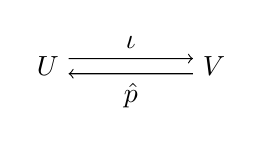
\begin{tikzpicture}[node distance = 6em, auto]
  \node (U) {$U$};
  \node (V) [right of = U] {$V$};
  \draw[->] (U.20) to node {$\iota$}(V.160);
  \draw[->] (V.200) to node {$\hat{p}$} (U.340);
 \end{tikzpicture}
\end{center}
where both maps are $G$-equivariant and $\hat{p} \iota = \id_U$. So the projection $\hat{p}$ splits and we obtain $V \cong U \oplus \ker \hat{p}$. Because $\hat{p}$ is $G$-equivariant $\ker \hat{p}$ is a subrepresentation of $V$. So $U$ has a complement which is again a representation.
\end{proof}

\begin{warn}
 The theorem is wrong in general if $\kchar k \mid |G|$. (An example will be on the exercise sheet.)
\end{warn}

\begin{expl}
 In general it is hard to compute a decomposition using Maschke’s theorem in practice!
 
 Let $G = S_3$. Let $V = kG$ be viewed as a representation of $G$ via the left multiplication, i.e.
 \[
  h.\left(\sum_{g \in G} a_g g\right) = \sum_{g \in G} a_g hg.
 \]
 Let $k = \C$, hence Maschke’s theorem holds. We want to find a decomposition of $kG$. Recall that $S_3 = \gen{s,t}$ where $s = (1 \; 2)$ and $t = (2 \; 3)$. We claim that
 \[
  kG = V_{\text{triv}} \oplus V_{\text{sgn}} \oplus V_1 \oplus V_2
 \]
 where
 \begin{align*}
  V_{\text{triv}} &\coloneqq \vspan\left(\sum_{g \in G} g \right) = \vspan(e+s+t+st+ts+sts), \\
  V_{\text{sgn}} &\coloneqq \vspan\left(e-s-t+st+ts-sts\right), \\
  V_1 &\coloneqq \vspan\left(e+s-ts, t+ts-st-sts\right) \text{ and} \\
  V_2 &\coloneqq \vspan\left(s+st-sts,e+t-s-st\right).
 \end{align*}
 Note that $G$ acts trivially on $V_{\text{triv}}$ and by multiplication with $-1$ on $V_{\text{sgn}}$ , hence $V_{\text{triv}}$ and $V_{\text{sgn}}$ are subrepresentations. One can also check that $V_1$ and $V_2$ are irreducible subrepresentations which are isomorphic.
\end{expl}


\begin{expl}
 Let $n \geq 2$ and $G = S_n$. Let $k$ be any field and let $S_n$ act on $k^n$ by setting
 \[
  g.e_i = e_{g(i)}
 \]
 where $e_1$, \dots, $e_n$ denotes the standard basis of $k^n$. Extending this linearly we get a representation of $G$ on $k^n$, i.e.
 \[
  g.(a_1, \dotsc, a_n) = \left(a_{g^{-1}(1)}, \dotsc, a_{g^{-1}(n)}\right).
 \]
 We can then set $V = k^n$ and extend the $G$-action on $V$ to be a $G$-action on $\mc{P}(V)$ by setting $(g.f)(v) = f(g^{-1}.v)$ for all $f \in \mc{P}(V), v \in V$. We can then ask ourselves how to describe $\mc{P}(V)$.
\end{expl}


\begin{defi}
 Let $k$ be a group and $W$ any $k$-vector space. Then $g.w = w$ for all $g \in G, w \in W$ defines a representation $W$ of $G$. This is called the \emph{trivial representation}. For each fixed dimension there is (up to isomorphism) one trivial representation. Therefore we usually say \emph{the} trivial representation of $G$ (of dimension $\dim W$).
\end{defi}


\begin{lem}
 Let $e_1$, \dots, $e_n$ denote the standard basis von $k^n$. $G = S_n$ acts linearly on $k^n$ as in the previous example.
 \begin{enumerate}[label=\emph{\alph*)},leftmargin=*]
  \item
   The vector subspaces
   \begin{gather*}
    U_1 \coloneqq \vspan\left( \sum_{i=1}^n e_i\right)
   \shortintertext{and}
    U_2 \coloneqq \left\{ (\lambda_1, \dotsc, \lambda_n) \in k^n \,\middle|\, \sum_{i=1}^n \lambda_i = 0 \right\}
   \end{gather*}
   are subrepresentations.
  \item
   $U_1$ is the trivial $1$-dimensional subrepresentation and
   \[
    \begin{cases}
     U_1 = U_2 & \text{if } n = 2, \kchar k = 2,\\
     U_1 \ncong U_2 & \text{otherwise}.
    \end{cases}
   \]
  \item
  If $n = 2$ then $V$ is completely reducible if and only if $\kchar k \neq 2$.
 \end{enumerate}
\end{lem}
\begin{proof}
 \begin{enumerate}[label=\emph{\alph*)},leftmargin=*]
  \item
   It is clear that $U_1$ and $U_2$ are vector subspaces. Since
   \[
    g.\left(\sum_{i=1}^n e_i\right)
    = \sum_{i=1}^n e_{g(i)}
    = \sum_{i=1}^n e_i
    \tag{$\ast$}
   \]
   we have $g.u \in U_1$ for all $g \in G, u \in U_1$, thus $U_1$ is a subrepresentation. Since
   \[
    g.(\lambda_1, \dotsc, \lambda_n) = \left( \lambda_{g^{-1}(1)}, \dotsc, \lambda_{g^{-1}(n)} \right)
   \]
   we have $g.u \in U_2$ for all $g \in G, u \in U_2$, thus $U_2$ is a subrepresentation.
  \item
   We have that $g.u = u$ for all $u \in U$ by ($\ast$).  If $n > 2$ then
   \[
    \dim U_1 = 1 \neq \dim U_2
   \]
   and thus $U_1 \ncong U_2$.
   
   If $n = 2$ and $S_2 = \{e,s\}$ then $s.(1,1) = (1,1)$ for the basis vector $(1,1)$ of $U_1$ and $s.(1,-1) = -(1,-1)$ for the basis vector $(1,-1)$ of $U_2$. So $U_2$ is not the trivial representation if $\kchar k \neq 2$, and thus $U_1 \ncong U_2$.  If $\kchar k = 2$ then $U_1$ and $U_2$ are both spanned by $(1,1)$ and thus $U_1 = U_2$.
  \item
   If $\kchar k \neq 2$ then $V$ is completely reducible by Maschke’s Theorem. If $\kchar k = 2$ then $U_1 = U_2$. This is the only one-dimensonal subrepresentation of $V$: If $U \subseteq V$ is a subrepresentation such that there exists $(\lambda, \mu) \in U$ with $\lambda \neq \mu$, then $(\mu, \lambda) \in U$ and thus $U = V$. Thus $V$ is indecomposible but reducible.
  \qedhere
 \end{enumerate}
\end{proof}


\begin{rem}
 In the case of $n = 2$ the representation $U_2$ is called the sign representation. More generally the sign representation of the symmetric group $S_n$ over a field $k$ is the (up to isomorphism unique) one-dimensional representation of $S_n$ over $k$ such that every $\sigma \in S_n$ acts by multiplication with $\sgn \sigma$. If $\kchar k = 2$ the sign representation coincides with the trivial representation of dimension $1$.
\end{rem}




